% CVPR 2022 Paper Template
% based on the CVPR template provided by Ming-Ming Cheng (https://github.com/MCG-NKU/CVPR_Template)
% modified and extended by Stefan Roth (stefan.roth@NOSPAMtu-darmstadt.de)

\documentclass[10pt,twocolumn,letterpaper]{article}

%%%%%%%%% PAPER TYPE  - PLEASE UPDATE FOR FINAL VERSION
\usepackage[review]{cvpr}      % To produce the REVIEW version
% \usepackage{cvpr}              % To produce the CAMERA-READY version
% \usepackage[xpagenumbers]{cvpr} % To force page numbers, e.g. for an arXiv version

% Include other packages here, before hyperref.
\usepackage{graphicx}
\usepackage{amsmath}
\usepackage{amssymb}
\usepackage{algorithm}
\usepackage{algpseudocode}
\usepackage{booktabs}
\usepackage{nicefrac}
\usepackage{xcolor,colortbl}
\usepackage{multirow}
\usepackage{sidecap}


\usepackage{pgfplots}
\DeclareUnicodeCharacter{2212}{−}
\usepgfplotslibrary{groupplots,dateplot}
\usetikzlibrary{patterns,shapes.arrows,external}
\pgfplotsset{compat=newest}
\usepackage{tikz}

\pgfplotsset{compat=1.11,
    /pgfplots/ybar legend/.style={
    /pgfplots/legend image code/.code={%
       \draw[##1,/tikz/.cd,yshift=-0.25em]
        (0cm,0cm) rectangle (3pt,0.8em);},
   },
}

\newcommand{\Karsten}[1]{\textcolor{red}{[Karsten: #1]}}
\newcommand{\Zeynep}[1]{\textcolor{magenta}{[Zeynep: #1]}}
\newcommand{\oriol}[1]{\textcolor{orange}{[Oriol: #1]}}
\newcommand{\red}[1]{\textcolor{red}{#1}}
\newcommand{\blue}[1]{\textcolor{blue}{#1}}

\DeclareMathOperator*{\argmax}{\arg\!\max}
\DeclareMathOperator*{\argmin}{\arg\!\min}

\definecolor{vvlightgray}{rgb}{0.9,0.9,0.9}
\definecolor{vlightgray}{rgb}{0.8,0.8,0.8}


% It is strongly recommended to use hyperref, especially for the review version.
% hyperref with option pagebackref eases the reviewers' job.
% Please disable hyperref *only* if you encounter grave issues, e.g. with the
% file validation for the camera-ready version.
%
% If you comment hyperref and then uncomment it, you should delete
% ReviewTempalte.aux before re-running LaTeX.
% (Or just hit 'q' on the first LaTeX run, let it finish, and you
%  should be clear).
\usepackage[pagebackref,breaklinks,colorlinks]{hyperref}


% Support for easy cross-referencing
\usepackage[capitalize]{cleveref}
\crefname{section}{Sec.}{Secs.}
\Crefname{section}{Section}{Sections}
\Crefname{table}{Table}{Tables}
\crefname{table}{Tab.}{Tabs.}

\newcommand{\zeynep}[1]{\textcolor{purple}{Zeynep: #1}}


%%%%%%%%% PAPER ID  - PLEASE UPDATE
\def\cvprPaperID{****} % *** Enter the CVPR Paper ID here
\def\confName{CVPR}
\def\confYear{2022}

\begin{document}

%%%%%%%%% TITLE - PLEASE UPDATE
\title{Learning fast, moving slow: \\Momentum-based Interpolation of Strong Zero-Shot Learners for Continual Learning}

\author{Authors}
\maketitle





%%%%%%%%%%%%%%%%%%%%%%%%%%%%%%%%%%%%%%%%%%%%%%%%%%%%%%%%%%%%%%%%%%%%%%%%
%%%%%%%%%%%%%%%%%%%%%%%%%%%%%%%%%%%%%%%%%%%%%%%%%%%%%%%%%%%%%%%%%%%%%%%%
\begin{abstract}
* Large pretrained, zero-shot capable models have shown considerable success both for standard transfer tasks, but recently also as a starting point for Continual Learning.\cite{?}
* However, these zero-shot models lose their benefits and robustness towards distribution shifts through naive finetuning.
* Continual Learning, where a consistent distribution shift is encountered, is there a tough task for standard zero-shot models.
* In this work, we showcase that where simple finetuning falls short, simple momentum-based weight interpolation can provide consistent improvements for Continual Learning tasks, for both memory-free and memory-based methods.
* We highlight that simple finetuning, and out-of-the-box zero-shot transfer performance, while easily outperforming existing methods not reliant on pretraining, can be improved significantly through continual learning with momentum-averaging.
* With the right adaptation, we find that momentum-based adaptation allows the continual learner to inch in parts very close to the joint training limits.
\end{abstract}









%%%%%%%%%%%%%%%%%%%%%%%%%%%%%%%%%%%%%%%%%%%%%%%%%%%%%%%%%%%%%%%%%%%%%%%%
%%%%%%%%%%%%%%%%%%%%%%%%%%%%%%%%%%%%%%%%%%%%%%%%%%%%%%%%%%%%%%%%%%%%%%%%
\section{Introduction}
* Quick introduction to Continual Learning
* Quick introduction to large pretrained models and strong zero-shot transfer.
* Hint to pretraining used in continual learning.
* Important: Hint that we ablate over smaller learning rates, so it is not just plain effective LR reduction.




%%%%%%%%%%%%%%%%%%%%%%%%%%%%%%%%%%%%%%%%%%%%%%%%%%%%%%%%%%%%%%%%%%%%%%%%
%%%%%%%%%%%%%%%%%%%%%%%%%%%%%%%%%%%%%%%%%%%%%%%%%%%%%%%%%%%%%%%%%%%%%%%%
\section{Related Work}
\textit{\textbf{Regularization-based methods}} augment the loss function with a regularization term that is intended to prevent forgetting by keeping the current parameters close to the parameters obtained during the past tasks. Elastic Weight Consolidation (EWC) \cite{doi:10.1073/pnas.1611835114} performs Laplace approximation on the posterior probabilities of the parameters of all previous task and uses the obtained means and covariance matrices to keep the current parameters close to the parameters of the previous tasks via the Mahalanobis distance. The more efficient \textbf{online Elastic Weight Consolidation (oEWC)}\cite{pmlr-v80-schwarz18a} suggests merely computing a momentum average of a single covariance matrix, and only keeping the parameters from the end of the previous task. Learning without Forgetting (LwF)\cite{8107520} also keeps the model parameters from the previous task and as a regularizer adds the cross-entropy between the class logits computed with the old weights and those with the current weights, using only data from the current task. Lastly, \cite{mirzadeh_2020_dropout} shows that using dropout as a regularizer forces the model to learn a gating mechanism such that for different tasks, different paths of the network are active.

\textit{\textbf{Rehearsal-based methods}} utilize Experience Replay \cite{pmid2186426} \cite{doi:10.1080/09540099550039318} by storing a small subset of the training data into a buffer, and continually replaying it as the model moves on to learn new tasks. \textbf{Dark Experience Replay (DER)} \cite{NEURIPS2020_b704ea2c} introduces regularization in the rehearsal scheme by matching the logits of the past with the logits computed by the current network parameters. Gradient Episodic Memory (GEM) \cite{NIPS2017_f8752278} and Average Gradient Episodic Memory (A-GEM) \cite{chaudhry2018efficient} enforce optimization constraints in the current task using data from past tasks. GDumb \cite{prabhu2020greedy} greedily stores samples in memory, and only trains the model at test time using merely samples from the buffer. DualNet \cite{NEURIPS2021_86a1fa88} uses a slow network for learning general task-agnostic features through Self-Supervised Learning, and a slow network for learning task-specific features for the problem at hand. Contrastive Continual Learning (Co2L) \cite{Cha_2021_ICCV} learns contrastive general task-agnostic features, and only at test time trains a linear classifier using data from the buffer.

\textit{\textbf{Flatness-seeking methods}} aim to locate and operate in flat minima regions for each task sequentially, thereby retaining performance on the old tasks. Finding Flat Minima (F2M) \cite{NEURIPS2021_357cfba1} proposes to independently add small random noise multiple times to the parameters in the pre-training procedure, thereby obtaining similar but different loss functions which are optimized together in order to locate flat minima. \cite{NEURIPS2020_518a38cc} studies how batch size, dropout and learning rate decay affect the model's ability to locate flat minima. Recently, \cite{mehta2021empirical} introduces the use of the Sharpness-Aware Minimization (SAM) \cite{foret2021sharpnessaware} procedure in continual learning, which explicitly optimizes for parameters lying in flat basins. Lastly, \textbf{Stochastic Weight Averaging (SWA)} \cite{izmailov2018averaging} demonstrates that averaging the weights of the model during training will implicitly land the final optimum in a flat region. Compared to the other flatness related approaches, SWA is only evaluated when the data stream is considered independent and identically distributed (IID). Given the aforementioned benefits of locating flat optima in a lifelong learning scenario, we aim to show that this approach can also substantially improve the performance when models are trained continually -- a typically non-IID learning setting. Nonetheless, this is an orthogonal method to not only all other categories of continual learning approaches, but also to the other flatness-seeking methods; for example \cite{DBLP:journals/corr/abs-2202-00661} demonstrates the benefits of combining both SAM and SWA when training on an IID stream of data.
% Intuitively, the model will spend a lot of time in flat basins due to small gradient updates; therefore, when averaging the weights of each gradient step we end up with parameters located near the most frequently visited spots in the loss landscape -- the flat minima.

%%%%%%%%%%%%%%%%%%%%%%%%%%%%%%%%%%%%%%%%%%%%%%%%%%%%%%%%%%%%%%%%%%%%%%%%
%%%%%%%%%%%%%%%%%%%%%%%%%%%%%%%%%%%%%%%%%%%%%%%%%%%%%%%%%%%%%%%%%%%%%%%%
\section{Method}
In this section we first cover the necessary preliminaries regarding a general Continual Learning (CL) problem, followed by an overview of our proposed method.
\subsection{Preliminaries}
The main goal of Continual Learning is to train a model $f_\theta$ on a sequence of $T$ tasks, such that for each task $t \in \{1, ..., T\}$ the learner gets access to a set of samples $D_t = \{(x_i, y_i)\}_{i=1}^{N_t}$. Formally, we solve the following optimization problem:
\begin{align*}
    \theta^{*} = \argmin_\theta \sum_{t=1}^T \mathbb{E}_{(x, y) \sim D_t} \left[L(f_\theta(x), y)\right]
\end{align*}

The difficulty comes from the imposed characteristic that at the time of learning task $t \in \{1, ..., T\}$, the model has no access to data from previous tasks $\tilde{t} \in \{1, ..., t-1\}$, therefore disregarding the typical IID (independent and identically distributed) assumption about the data. Memory-based approaches impose a slight relaxation on this property, by allowing the model to store a small buffer of samples.

\begin{algorithm}
\caption{Momentum-based Continual Learning (MCL)}\label{alg:mcl}
\begin{algorithmic}[1]
\Require Pre-trained weights $\theta_{pre}$, Momentum $\tau \in [0, 1]$ 
\State $\theta \gets \theta_{pre}$
\State $\theta_{slow} \gets \theta_{pre}$
\For{$t \gets 1$ \ldots num\_tasks}
    \For{$e \gets 1$ \ldots num\_epochs}   
        \For{$(x, y) \sim D_t$}   
            \State{$\theta \gets \theta - \alpha \nabla \mathcal{L}(f_\theta(x), y)$}
            \State{$\theta_{slow} \gets \tau \cdot \theta_{slow} + (1-\tau) \cdot \theta$}
        \EndFor
    \EndFor
\EndFor
\State $\theta \gets \theta_{slow}$
\end{algorithmic}
\end{algorithm}

\subsection{Momentum-based Continual Learning (MCL)}
Recently, Stochastic Weighted Averaging (SWA) \cite{izmailov2018averaging} demonstrated that fine-tuning a pre-trained model by retaining a running average of the weights leads to wider optima and better generalization performance. Nevertheless, this work has primarily focused on the context of IID data, and hasn't yet explored the capabilities of the approach when applied to a non-IID stream of data, such as the one typically seen in Continual Learning. \\

Given that several works \cite{NEURIPS2021_357cfba1} \cite{NEURIPS2020_518a38cc} \cite{foret2021sharpnessaware} in the Continual Learning literature have focused on the benefits of optimizing for flat minima, we aim to explore whether the implicit flat-finding minima procedure of SWA is beneficial for life-long learning.\\

To this end we introduce a reformulation of SWA named \textbf{Momentum-based Continual Learning (MCL)}, with the goal of estimating how well a model performs in a continual learning setting when keeping an exponential moving average of the weights. A simplified version of the MCL procedure is summarized in Algorithm \ref{alg:mcl}. \\

Note that MCL doesn't resemble a typical continual learning method, which commonly incorporates a memory buffer, a loss regularization, and/or dependency on explicit task boundaries. This approach can be neatly packed into an optimizer, and in fact be used orthogonal to any of the existing continual learning methods. \\

On a more abstract level, our approach also builds upon the Complimentary Learning Systems (CLS) \cite{pmid7624455} theory from neuroscience, which essentially states that humans are capable of learning continually with the help of two complimentary systems: A \textit{fast} learning system, which allows for rapidly learning new experiences via synaptic changes in the hippocamal system; and a \textit{slow} learning system which gradually integrates these new experiences in the ensemble of past observations stored in the neocortical memory system.



%%%%%%%%%%%%%%%%%%%%%%%%%%%%%%%%%%%%%%%%%%%%%%%%%%%%%%%%%%%%%%%%%%%%%%%%
%%%%%%%%%%%%%%%%%%%%%%%%%%%%%%%%%%%%%%%%%%%%%%%%%%%%%%%%%%%%%%%%%%%%%%%%
\section{Experiments}
This section provides details regarding the evaluation protocol (Section \ref{sec:evaluation-protocol}), followed by an analysis of the obtained experimental results (Section \ref{sec:experimental-results}), concluded by an ablation study of the hyperparameters (Section \ref{sec:ablation-study}).

\subsection{Evaluation protocol} \label{sec:evaluation-protocol}
\textbf{Datasets.} For the purpose of evaluating the proposed method, we provide benchmarks on three datasets commonly used in the continual learning literature: CIFAR-10 \cite{Krizhevsky09learningmultiple}, CIFAR-100 \cite{Krizhevsky09learningmultiple}, and Tiny ImageNet. In order to train and evaluate the methods in a continual manner, we split each dataset in several tasks, in a way that each sequential task contains non-overlapping classes. More precisely, Seq-CIFAR-10 consists of 5 tasks (each containing 2 classes), Seq-CIFAR-100 consists of 10 tasks (each containing 10 classes), and Seq-Tiny-ImageNet consists of 10 tasks (each containing 20 classes). 

\textbf{Continual Learning protocols.}  We consider two standard continual frameworks of evaluation: Task Incremental Learning (Task-IL) and Class Incremental Learning (Class-IL). The main difference is that the former provides task identities at prediction time, meaning that the model only has to choose between the classes for the given task; whereas in the latter case the model is free to make predictions for classes outside the current task, thereby being much more susceptible to making mistakes. 


\textbf{Model architecture. } For all three datasets (CIFAR-10, CIFAR-100, Tiny ImageNet), we fine-tune the pre-trained architecture of CLIP \cite{pmlr-v139-radford21a} which uses ViT-B/16 as the image processing network. 


\textbf{Training. } In order to minimize the potential factors of variation, for all methods and all datasets we use the standard SGD \cite{pmlr-v28-shamir13} optimizer with a fixed learning rate and no scheduler, as well as a fixed number of epochs set to $10$. Before evaluating on the test set, we perform a grid search on a hold-out validation set, which is obtained by randomly sampling $10\%$ of the train set. More precisely, we search for the best learning rate among the set $\{10^{-2}, 10^{-3}, 10^{-4}, 10^{-5}, 10^{-6}, 10^{-7}\}$, and for the best $\tau$ parameter among the set $\{0.995, 0.997, 0.999, 0.9995, 0.9997, 0.9999 \}$. 

\textbf{Code. } We build our method on top of the implementation open-sourced by \cite{NEURIPS2020_b704ea2c}, where the authors implement a large variety of Continual Learning methods and benchmarks in PyTorch \cite{NEURIPS2019_9015}. 

\subsection{Experimental Results}  \label{sec:experimental-results}
We compare the use of Momentum in three standard continual learning categories: fine-tuning (pure SGD \cite{pmlr-v28-shamir13}), regularization-based (oEWC \cite{pmlr-v80-schwarz18a}), and rehearsal-based (DER++ \cite{NEURIPS2020_b704ea2c} with buffer size $500$ and $5000$). All results presented below are obtained by averaging the runs over three seeds, where the standard deviation is provided as confidence bound. \\\\
First, we provide a lower bound by evaluating the model in a zero-shot setting, as well as an upper bound by training it on all tasks jointly (see Table \ref{table-baselines}). It should be noted that since the joint training is evaluated without providing task boundaries, the Task-IL scenario might actually outperform this upper bound. \\\\
The results of evaluating the methods in a Continual Learning scenario are summarized in Table \ref{table-continual}. We empirically show that keeping a momentum-updated version of the network trained with either of the three prototypical methods (pure SGD, regularization-based, and rehearsal-based) results in consistent improvement over the baseline. We argue that this is due to the ability of the momentum network to converge to flatter minima, thereby displaying better generalization performance on both old and new tasks. \\\\
We hypothesize that the improvements on Seq-CIFAR-10 are marginal because this is a fairly easy continual learning benchmark by today's standards (5 tasks, with 2 classes each), and thereby there is not much room for improvement over the baselines. Nevertheless, as we move towards harder datasets with increased class diversity and longer task sequences, such as those in Seq-CIFAR-100 and Seq-Tiny-ImageNet, the gap between between using momentum or not significantly increases. \\\\
Interestingly, we observe that momentum based DER++ with a buffer size of 500 almost closes the gap in performance compared to the non-momentum based DER++ with buffer size 5000. Following are the aforementioned gaps for the Class-IL scenario, with the difference for the non-momentum based DER++ with buffer size of 500 denoted in parentheses: $1.35 \%$ ($2.43 \%$) on Seq-CIFAR-10, $1.15 \%$ ($6.48 \%$) on Seq-CIFAR-100, and $1.43 \%$ ($5.49 \%$) on Seq-Tiny-ImageNet. The improvement in performance by going from non-momentum to momentum based alternative is evident. In doing so, this demonstrates that the need for buffer size can decrease significantly (in this case, 10-fold) when one merely keeps a running average copy of the network. \\\\
Finally, we would like to point out that training momentum-based DER++ with a buffer of 5000 in Class-IL setting even further closes the gap to the upper bound denoted by the joint setting. Following are the gaps to the upper bound, with the difference for non-momentum based DER++ with buffer size of 5000 denoted in parentheses: $0.32 \%$ ($0.45 \%$) on Seq-CIFAR-10, $2.28 \%$ ($4.06 \%$) on Seq-CIFAR-100, and $0.6 \%$ ($2.32 \%$) on Seq-Tiny-ImageNet. Again, the empirical results clearly indicate that keeping a running average copy of the network is beneficial across a variety of benchmarks, and helps further close the gap to the upper bound performance.

\subsection{Ablation study}
\label{sec:ablation-study}
\textbf{Momentum strength. } In Figure \ref{fig:tau_class-il-acc} we show how the momentum strength $\tau$ affects the model's Class-IL Accuracy. While we find that the optimal value of $\tau$ is dataset-dependent, it is encouraging that the vastly different methods show surprisingly similar behavior across the examined range of $\tau$ for a given dataset.

\textbf{Restart frequency. } Next, we examine whether it is beneficial to occasionally restart the fast weights $\theta$ with the slow weights $\theta_{slow}$ during the training procedure. To this end, we introduce a new hyperparameter \textit{restart frequency} which specifies after how many gradient steps we perform the aforementioned restart. From the results detailed in Figure \ref{fig:restats}, we find that restarting the fast weights is not beneficial to the training procedure.

\textbf{Update frequency. } Finally, we examine whether it is beneficial to perform the update of the slow weights (Line 7 in Algorithm \ref{alg:mcl}) at various update frequencies. For this purpose, we introduce a new hyperparameter \textit{update frequency} which specifies after how many gradient steps we perform the update of the slow weights. From the results summarized in Figure \ref{fig:updates}, we find that updating at frequencies higher than 1 (where 1 is the default behavior of our algorithm) does not provide a boost in performance.

\begin{table*}[t]
  \caption{\textit{Baseline setting} -- training and evaluating on all tasks jointly.}
  \label{table-baselines}
  \centering
  \begin{tabular}{cccc}
    \toprule
    \textbf{Baseline} & \textbf{CIFAR-10} & \textbf{CIFAR-100} & \textbf{Tiny-ImageNet} \\ 
    \midrule 
    ZERO-SHOT & $88.77$ & $63.11$ & $58.53$ \\ 
    JOINT & $97.53 \pm 0.08$ & $87.22 \pm 0.54$ & $78.86 \pm 1.38$ \\
    \bottomrule
  \end{tabular}
\end{table*}

\begin{table*}[t]
  \caption{\textit{Continual learning setting} -- training and evaluating on sequences of tasks.}
  \label{table-continual}
  \centering
  \begin{tabular}{cccccccccc}
    \toprule
    \multirow{2}{*}{\textbf{Method}} & \multirow{2}{*}{\textbf{Momentum}}  & \multicolumn{2}{c}{\textbf{Seq-CIFAR-10}}  & \multicolumn{2}{c}{\textbf{Seq-CIFAR-100}}  & \multicolumn{2}{c}{\textbf{Seq-Tiny-ImageNet}} \\
    & & Class-IL & Task-IL & Class-IL & Task-IL & Class-IL & Task-IL \\
    \midrule 
    
    \multirow{2}{*}{SGD} & no & $91.38 \pm 0.04$ & $98.17 \pm 0.01$ & $74.36 \pm 0.03$ & $93.59 \pm 0.04$ & $67.30 \pm 0.08$ & $82.12 \pm 0.07$ \\
     & yes & $92.46 \pm 0.11$ & $98.43 \pm 0.01$ & $77.52 \pm 0.37$ & $94.98 \pm 0.17$ & $71.09 \pm 0.28$ & $85.22 \pm 0.32$ \\
    \midrule

    \multirow{2}{*}{oEWC} & no & $90.67 \pm 0.01$ & $98.17 \pm 0.01$ & $74.07 \pm 0.20$ & $93.80 \pm 0.02$ & $66.60 \pm 0.02$ & $81.79 \pm 0.02$ \\
     & yes & $91.87 \pm 0.57$ & $98.88 \pm 0.12$ & $77.25 \pm 0.31$ & $95.09 \pm 0.01$ & $71.57 \pm 0.05$ & $85.94 \pm 0.07$ \\
    \midrule

    \multirow{2}{*}{DER++ (500)} & no & $94.65 \pm 0.16$ & $99.38 \pm 0.10$ & $76.68 \pm 0.23$ & $95.05 \pm 0.09$ & $71.05 \pm 0.12$ & $84.42 \pm 0.22$ \\
     & yes & $95.73 \pm 0.21$ & $99.50 \pm 0.04$ & $82.01 \pm 0.31$ & $96.69 \pm 0.03$ & $75.11 \pm 0.02$ & $87.80 \pm 0.27$ \\
    \midrule

    \multirow{2}{*}{DER++ (5000)} & no & $97.08 \pm 0.04$ & $99.60 \pm 0.01$ & $83.16 \pm 0.20$ & $97.03 \pm 0.11$ & $76.54 \pm 0.10$ & $88.44 \pm 0.04$ \\
     & yes & $97.21 \pm 0.11$ & $99.62 \pm 0.01$ & $84.94 \pm 0.07$ & $97.13 \pm 0.05$ & $78.26 \pm 0.14$ & $89.00 \pm 0.11$ \\

    \bottomrule
  \end{tabular}
\end{table*}

% \begin{figure}[htb!]
% \centering
% \resizebox{2cm}{!}{% This file was created with tikzplotlib v0.10.1.
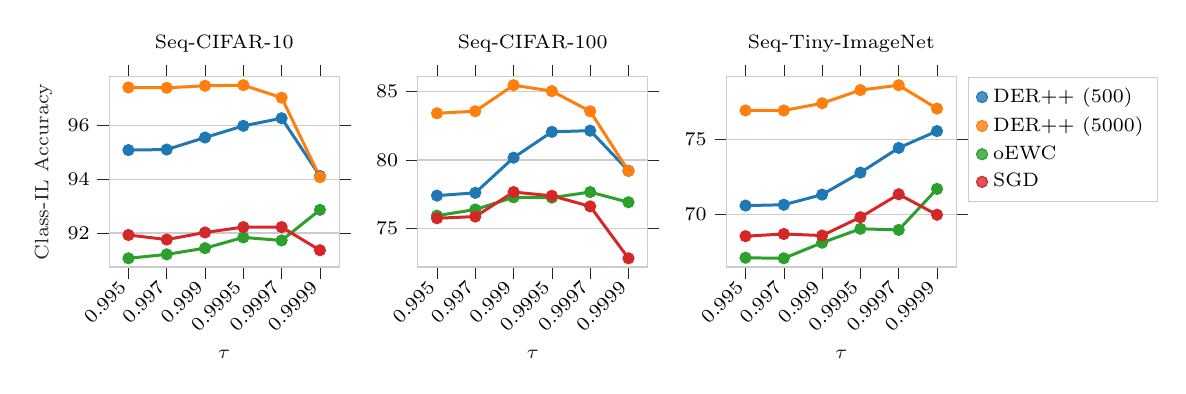
\begin{tikzpicture}
\scriptsize
\definecolor{crimson2143940}{RGB}{214,39,40}
\definecolor{darkorange25512714}{RGB}{255,127,14}
\definecolor{darkslategray38}{RGB}{38,38,38}
\definecolor{forestgreen4416044}{RGB}{44,160,44}
\definecolor{lightgray204}{RGB}{204,204,204}
\definecolor{steelblue31119180}{RGB}{31,119,180}



\begin{groupplot}[
    group style={group size=3 by 1},
    width=4.5cm,
    height=4cm
]

\nextgroupplot[
axis line style={lightgray204},
tick align=outside,
title={Seq-CIFAR-10},
unbounded coords=jump,
x grid style={lightgray204},
xlabel=\textcolor{darkslategray38}{$\tau$},
xmajorticks=true,
xmin=-0.5, xmax=5.5,
xtick style={color=darkslategray38},
xticklabel style={rotate=45,anchor=east},
xtick={0,1,2,3,4,5},
% xtick style={}
xticklabels={0.995,0.997,0.999,0.9995,0.9997,0.9999},
y grid style={lightgray204},
ylabel=\textcolor{darkslategray38}{Class-IL Accuracy},
ymajorgrids,
ymajorticks=true,
ymin=90.7385, ymax=97.8115,
ytick style={color=darkslategray38}
]
\addplot [line width=1.08pt, steelblue31119180]
table {%
0 95.08
1 95.1
2 95.5466666666667
3 95.98
4 96.2633333333333
5 94.1166666666667
};
\addplot [line width=1.08pt, steelblue31119180]
table {%
0 nan
0 nan
};
\addplot [line width=1.08pt, steelblue31119180]
table {%
1 nan
1 nan
};
\addplot [line width=1.08pt, steelblue31119180]
table {%
2 nan
2 nan
};
\addplot [line width=1.08pt, steelblue31119180]
table {%
3 nan
3 nan
};
\addplot [line width=1.08pt, steelblue31119180]
table {%
4 nan
4 nan
};
\addplot [line width=1.08pt, steelblue31119180]
table {%
5 nan
5 nan
};
\addplot [draw=steelblue31119180, fill=steelblue31119180, mark=*, only marks]
table{%
x  y
0 95.08
1 95.1
2 95.5466666666667
3 95.98
4 96.2633333333333
5 94.1166666666667
};
\addplot [line width=1.08pt, darkorange25512714]
table {%
0 97.4066666666667
1 97.3933333333333
2 97.4666666666667
3 97.49
4 97.0266666666667
5 94.0766666666667
};
\addplot [line width=1.08pt, darkorange25512714]
table {%
0 nan
0 nan
};
\addplot [line width=1.08pt, darkorange25512714]
table {%
1 nan
1 nan
};
\addplot [line width=1.08pt, darkorange25512714]
table {%
2 nan
2 nan
};
\addplot [line width=1.08pt, darkorange25512714]
table {%
3 nan
3 nan
};
\addplot [line width=1.08pt, darkorange25512714]
table {%
4 nan
4 nan
};
\addplot [line width=1.08pt, darkorange25512714]
table {%
5 nan
5 nan
};
\addplot [draw=darkorange25512714, fill=darkorange25512714, mark=*, only marks]
table{%
x  y
0 97.4066666666667
1 97.3933333333333
2 97.4666666666667
3 97.49
4 97.0266666666667
5 94.0766666666667
};
\addplot [line width=1.08pt, forestgreen4416044]
table {%
0 91.06
1 91.2066666666667
2 91.4366666666667
3 91.8366666666667
4 91.7233333333333
5 92.86
};
\addplot [line width=1.08pt, forestgreen4416044]
table {%
0 nan
0 nan
};
\addplot [line width=1.08pt, forestgreen4416044]
table {%
1 nan
1 nan
};
\addplot [line width=1.08pt, forestgreen4416044]
table {%
2 nan
2 nan
};
\addplot [line width=1.08pt, forestgreen4416044]
table {%
3 nan
3 nan
};
\addplot [line width=1.08pt, forestgreen4416044]
table {%
4 nan
4 nan
};
\addplot [line width=1.08pt, forestgreen4416044]
table {%
5 nan
5 nan
};
\addplot [draw=forestgreen4416044, fill=forestgreen4416044, mark=*, only marks]
table{%
x  y
0 91.06
1 91.2066666666667
2 91.4366666666667
3 91.8366666666667
4 91.7233333333333
5 92.86
};
\addplot [line width=1.08pt, crimson2143940]
table {%
0 91.9266666666667
1 91.7566666666667
2 92.02
3 92.22
4 92.22
5 91.36
};
\addplot [line width=1.08pt, crimson2143940]
table {%
0 nan
0 nan
};
\addplot [line width=1.08pt, crimson2143940]
table {%
1 nan
1 nan
};
\addplot [line width=1.08pt, crimson2143940]
table {%
2 nan
2 nan
};
\addplot [line width=1.08pt, crimson2143940]
table {%
3 nan
3 nan
};
\addplot [line width=1.08pt, crimson2143940]
table {%
4 nan
4 nan
};
\addplot [line width=1.08pt, crimson2143940]
table {%
5 nan
5 nan
};
\addplot [draw=crimson2143940, fill=crimson2143940, mark=*, only marks]
table{%
x  y
0 91.9266666666667
1 91.7566666666667
2 92.02
3 92.22
4 92.22
5 91.36
};

\nextgroupplot[
axis line style={lightgray204},
tick align=outside,
title={Seq-CIFAR-100},
unbounded coords=jump,
x grid style={lightgray204},
xlabel=\textcolor{darkslategray38}{$\tau$},
xmajorticks=true,
xmin=-0.5, xmax=5.5,
xtick style={color=darkslategray38},
xtick={0,1,2,3,4,5},
xticklabels={0.995,0.997,0.999,0.9995,0.9997,0.9999},
xticklabel style={rotate=45,anchor=east},
y grid style={lightgray204},
% ylabel=\textcolor{darkslategray38}{Class-IL Accuracy},
ymajorgrids,
ymajorticks=true,
ymin=72.2023333333333, ymax=86.0843333333333,
ytick style={color=darkslategray38}
]
\addplot [line width=1.08pt, steelblue31119180]
table {%
0 77.4033333333333
1 77.6066666666667
2 80.17
3 82.0533333333333
4 82.14
5 79.2166666666667
};
\addplot [line width=1.08pt, steelblue31119180]
table {%
0 nan
0 nan
};
\addplot [line width=1.08pt, steelblue31119180]
table {%
1 nan
1 nan
};
\addplot [line width=1.08pt, steelblue31119180]
table {%
2 nan
2 nan
};
\addplot [line width=1.08pt, steelblue31119180]
table {%
3 nan
3 nan
};
\addplot [line width=1.08pt, steelblue31119180]
table {%
4 nan
4 nan
};
\addplot [line width=1.08pt, steelblue31119180]
table {%
5 nan
5 nan
};
\addplot [draw=steelblue31119180, fill=steelblue31119180, mark=*, only marks]
table{%
x  y
0 77.4033333333333
1 77.6066666666667
2 80.17
3 82.0533333333333
4 82.14
5 79.2166666666667
};
\addplot [line width=1.08pt, darkorange25512714]
table {%
0 83.4066666666667
1 83.5566666666667
2 85.4533333333333
3 85.0233333333333
4 83.5533333333333
5 79.2
};
\addplot [line width=1.08pt, darkorange25512714]
table {%
0 nan
0 nan
};
\addplot [line width=1.08pt, darkorange25512714]
table {%
1 nan
1 nan
};
\addplot [line width=1.08pt, darkorange25512714]
table {%
2 nan
2 nan
};
\addplot [line width=1.08pt, darkorange25512714]
table {%
3 nan
3 nan
};
\addplot [line width=1.08pt, darkorange25512714]
table {%
4 nan
4 nan
};
\addplot [line width=1.08pt, darkorange25512714]
table {%
5 nan
5 nan
};
\addplot [draw=darkorange25512714, fill=darkorange25512714, mark=*, only marks]
table{%
x  y
0 83.4066666666667
1 83.5566666666667
2 85.4533333333333
3 85.0233333333333
4 83.5533333333333
5 79.2
};
\addplot [line width=1.08pt, forestgreen4416044]
table {%
0 75.9433333333333
1 76.39
2 77.28
3 77.2566666666667
4 77.6633333333333
5 76.92
};
\addplot [line width=1.08pt, forestgreen4416044]
table {%
0 nan
0 nan
};
\addplot [line width=1.08pt, forestgreen4416044]
table {%
1 nan
1 nan
};
\addplot [line width=1.08pt, forestgreen4416044]
table {%
2 nan
2 nan
};
\addplot [line width=1.08pt, forestgreen4416044]
table {%
3 nan
3 nan
};
\addplot [line width=1.08pt, forestgreen4416044]
table {%
4 nan
4 nan
};
\addplot [line width=1.08pt, forestgreen4416044]
table {%
5 nan
5 nan
};
\addplot [draw=forestgreen4416044, fill=forestgreen4416044, mark=*, only marks]
table{%
x  y
0 75.9433333333333
1 76.39
2 77.28
3 77.2566666666667
4 77.6633333333333
5 76.92
};
\addplot [line width=1.08pt, crimson2143940]
table {%
0 75.7533333333333
1 75.8766666666667
2 77.6633333333333
3 77.39
4 76.62
5 72.8333333333333
};
\addplot [line width=1.08pt, crimson2143940]
table {%
0 nan
0 nan
};
\addplot [line width=1.08pt, crimson2143940]
table {%
1 nan
1 nan
};
\addplot [line width=1.08pt, crimson2143940]
table {%
2 nan
2 nan
};
\addplot [line width=1.08pt, crimson2143940]
table {%
3 nan
3 nan
};
\addplot [line width=1.08pt, crimson2143940]
table {%
4 nan
4 nan
};
\addplot [line width=1.08pt, crimson2143940]
table {%
5 nan
5 nan
};
\addplot [draw=crimson2143940, fill=crimson2143940, mark=*, only marks]
table{%
x  y
0 75.7533333333333
1 75.8766666666667
2 77.6633333333333
3 77.39
4 76.62
5 72.8333333333333
};

\nextgroupplot[
axis line style={lightgray204},
legend cell align={left},
legend style={
  fill opacity=0.8,
  draw opacity=1,
  text opacity=1,
  at={(1.05,1)},
  anchor=north west,
  draw=lightgray204
},
tick align=outside,
title={Seq-Tiny-ImageNet},
unbounded coords=jump,
x grid style={lightgray204},
xlabel=\textcolor{darkslategray38}{$\tau$},
xmajorticks=true,
xmin=-0.5, xmax=5.5,
xtick style={color=darkslategray38},
xticklabel style={rotate=45,anchor=east},
xtick={0,1,2,3,4,5},
xticklabels={0.995,0.997,0.999,0.9995,0.9997,0.9999},
y grid style={lightgray204},
% ylabel=\textcolor{darkslategray38}{Class-IL Accuracy},
ymajorgrids,
ymajorticks=true,
ymin=66.4991666666667, ymax=79.2041666666667,
ytick style={color=darkslategray38}
]
\addplot [line width=1.08pt, steelblue31119180, forget plot]
table {%
0 70.5933333333333
1 70.65
2 71.3266666666667
3 72.7933333333333
4 74.4433333333333
5 75.5666666666667
};
\addplot [line width=1.08pt, steelblue31119180, forget plot]
table {%
0 nan
0 nan
};
\addplot [line width=1.08pt, steelblue31119180, forget plot]
table {%
1 nan
1 nan
};
\addplot [line width=1.08pt, steelblue31119180, forget plot]
table {%
2 nan
2 nan
};
\addplot [line width=1.08pt, steelblue31119180, forget plot]
table {%
3 nan
3 nan
};
\addplot [line width=1.08pt, steelblue31119180, forget plot]
table {%
4 nan
4 nan
};
\addplot [line width=1.08pt, steelblue31119180, forget plot]
table {%
5 nan
5 nan
};
\addplot [draw=steelblue31119180, fill=steelblue31119180, mark=*, only marks]
table{%
x  y
0 70.5933333333333
1 70.65
2 71.3266666666667
3 72.7933333333333
4 74.4433333333333
5 75.5666666666667
};
\addlegendentry{DER++ (500)}
\addplot [line width=1.08pt, darkorange25512714, forget plot]
table {%
0 76.9433333333333
1 76.94
2 77.42
3 78.3
4 78.6266666666667
5 77.0633333333333
};
\addplot [line width=1.08pt, darkorange25512714, forget plot]
table {%
0 nan
0 nan
};
\addplot [line width=1.08pt, darkorange25512714, forget plot]
table {%
1 nan
1 nan
};
\addplot [line width=1.08pt, darkorange25512714, forget plot]
table {%
2 nan
2 nan
};
\addplot [line width=1.08pt, darkorange25512714, forget plot]
table {%
3 nan
3 nan
};
\addplot [line width=1.08pt, darkorange25512714, forget plot]
table {%
4 nan
4 nan
};
\addplot [line width=1.08pt, darkorange25512714, forget plot]
table {%
5 nan
5 nan
};
\addplot [draw=darkorange25512714, fill=darkorange25512714, mark=*, only marks]
table{%
x  y
0 76.9433333333333
1 76.94
2 77.42
3 78.3
4 78.6266666666667
5 77.0633333333333
};
\addlegendentry{DER++ (5000)}
\addplot [line width=1.08pt, forestgreen4416044, forget plot]
table {%
0 67.1133333333333
1 67.0766666666667
2 68.1166666666667
3 69.0466666666667
4 68.97
5 71.7066666666667
};
\addplot [line width=1.08pt, forestgreen4416044, forget plot]
table {%
0 nan
0 nan
};
\addplot [line width=1.08pt, forestgreen4416044, forget plot]
table {%
1 nan
1 nan
};
\addplot [line width=1.08pt, forestgreen4416044, forget plot]
table {%
2 nan
2 nan
};
\addplot [line width=1.08pt, forestgreen4416044, forget plot]
table {%
3 nan
3 nan
};
\addplot [line width=1.08pt, forestgreen4416044, forget plot]
table {%
4 nan
4 nan
};
\addplot [line width=1.08pt, forestgreen4416044, forget plot]
table {%
5 nan
5 nan
};
\addplot [draw=forestgreen4416044, fill=forestgreen4416044, mark=*, only marks]
table{%
x  y
0 67.1133333333333
1 67.0766666666667
2 68.1166666666667
3 69.0466666666667
4 68.97
5 71.7066666666667
};
\addlegendentry{oEWC}
\addplot [line width=1.08pt, crimson2143940, forget plot]
table {%
0 68.5533333333333
1 68.7
2 68.5966666666667
3 69.8166666666667
4 71.35
5 69.9833333333333
};
\addplot [line width=1.08pt, crimson2143940, forget plot]
table {%
0 nan
0 nan
};
\addplot [line width=1.08pt, crimson2143940, forget plot]
table {%
1 nan
1 nan
};
\addplot [line width=1.08pt, crimson2143940, forget plot]
table {%
2 nan
2 nan
};
\addplot [line width=1.08pt, crimson2143940, forget plot]
table {%
3 nan
3 nan
};
\addplot [line width=1.08pt, crimson2143940, forget plot]
table {%
4 nan
4 nan
};
\addplot [line width=1.08pt, crimson2143940, forget plot]
table {%
5 nan
5 nan
};
\addplot [draw=crimson2143940, fill=crimson2143940, mark=*, only marks]
table{%
x  y
0 68.5533333333333
1 68.7
2 68.5966666666667
3 69.8166666666667
4 71.35
5 69.9833333333333
};
\addlegendentry{SGD}
\end{groupplot}

\end{tikzpicture}
}
% \caption{my figure drawn in tikz}\label{fig:myfigure}
% \end{figure}



\begin{figure*}[ht!]
    \centering
    % This file was created with tikzplotlib v0.10.1.
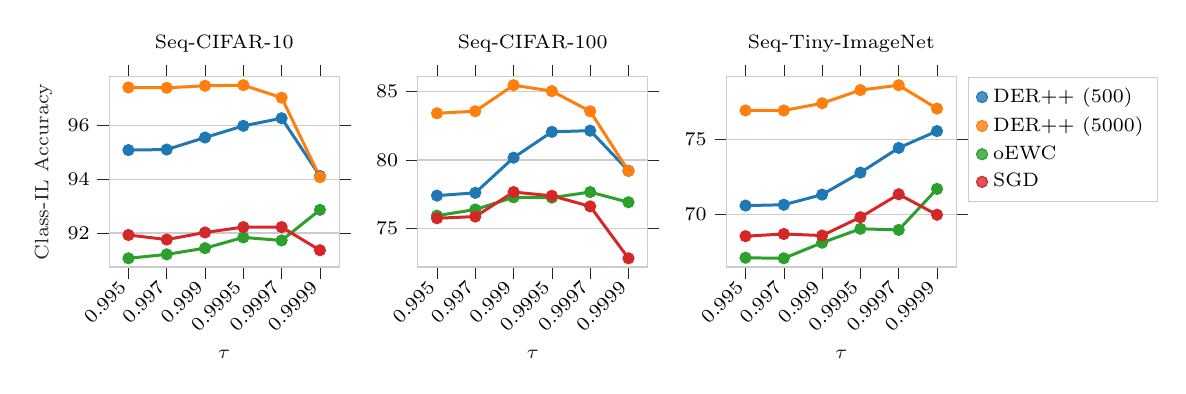
\begin{tikzpicture}
\scriptsize
\definecolor{crimson2143940}{RGB}{214,39,40}
\definecolor{darkorange25512714}{RGB}{255,127,14}
\definecolor{darkslategray38}{RGB}{38,38,38}
\definecolor{forestgreen4416044}{RGB}{44,160,44}
\definecolor{lightgray204}{RGB}{204,204,204}
\definecolor{steelblue31119180}{RGB}{31,119,180}



\begin{groupplot}[
    group style={group size=3 by 1},
    width=4.5cm,
    height=4cm
]

\nextgroupplot[
axis line style={lightgray204},
tick align=outside,
title={Seq-CIFAR-10},
unbounded coords=jump,
x grid style={lightgray204},
xlabel=\textcolor{darkslategray38}{$\tau$},
xmajorticks=true,
xmin=-0.5, xmax=5.5,
xtick style={color=darkslategray38},
xticklabel style={rotate=45,anchor=east},
xtick={0,1,2,3,4,5},
% xtick style={}
xticklabels={0.995,0.997,0.999,0.9995,0.9997,0.9999},
y grid style={lightgray204},
ylabel=\textcolor{darkslategray38}{Class-IL Accuracy},
ymajorgrids,
ymajorticks=true,
ymin=90.7385, ymax=97.8115,
ytick style={color=darkslategray38}
]
\addplot [line width=1.08pt, steelblue31119180]
table {%
0 95.08
1 95.1
2 95.5466666666667
3 95.98
4 96.2633333333333
5 94.1166666666667
};
\addplot [line width=1.08pt, steelblue31119180]
table {%
0 nan
0 nan
};
\addplot [line width=1.08pt, steelblue31119180]
table {%
1 nan
1 nan
};
\addplot [line width=1.08pt, steelblue31119180]
table {%
2 nan
2 nan
};
\addplot [line width=1.08pt, steelblue31119180]
table {%
3 nan
3 nan
};
\addplot [line width=1.08pt, steelblue31119180]
table {%
4 nan
4 nan
};
\addplot [line width=1.08pt, steelblue31119180]
table {%
5 nan
5 nan
};
\addplot [draw=steelblue31119180, fill=steelblue31119180, mark=*, only marks]
table{%
x  y
0 95.08
1 95.1
2 95.5466666666667
3 95.98
4 96.2633333333333
5 94.1166666666667
};
\addplot [line width=1.08pt, darkorange25512714]
table {%
0 97.4066666666667
1 97.3933333333333
2 97.4666666666667
3 97.49
4 97.0266666666667
5 94.0766666666667
};
\addplot [line width=1.08pt, darkorange25512714]
table {%
0 nan
0 nan
};
\addplot [line width=1.08pt, darkorange25512714]
table {%
1 nan
1 nan
};
\addplot [line width=1.08pt, darkorange25512714]
table {%
2 nan
2 nan
};
\addplot [line width=1.08pt, darkorange25512714]
table {%
3 nan
3 nan
};
\addplot [line width=1.08pt, darkorange25512714]
table {%
4 nan
4 nan
};
\addplot [line width=1.08pt, darkorange25512714]
table {%
5 nan
5 nan
};
\addplot [draw=darkorange25512714, fill=darkorange25512714, mark=*, only marks]
table{%
x  y
0 97.4066666666667
1 97.3933333333333
2 97.4666666666667
3 97.49
4 97.0266666666667
5 94.0766666666667
};
\addplot [line width=1.08pt, forestgreen4416044]
table {%
0 91.06
1 91.2066666666667
2 91.4366666666667
3 91.8366666666667
4 91.7233333333333
5 92.86
};
\addplot [line width=1.08pt, forestgreen4416044]
table {%
0 nan
0 nan
};
\addplot [line width=1.08pt, forestgreen4416044]
table {%
1 nan
1 nan
};
\addplot [line width=1.08pt, forestgreen4416044]
table {%
2 nan
2 nan
};
\addplot [line width=1.08pt, forestgreen4416044]
table {%
3 nan
3 nan
};
\addplot [line width=1.08pt, forestgreen4416044]
table {%
4 nan
4 nan
};
\addplot [line width=1.08pt, forestgreen4416044]
table {%
5 nan
5 nan
};
\addplot [draw=forestgreen4416044, fill=forestgreen4416044, mark=*, only marks]
table{%
x  y
0 91.06
1 91.2066666666667
2 91.4366666666667
3 91.8366666666667
4 91.7233333333333
5 92.86
};
\addplot [line width=1.08pt, crimson2143940]
table {%
0 91.9266666666667
1 91.7566666666667
2 92.02
3 92.22
4 92.22
5 91.36
};
\addplot [line width=1.08pt, crimson2143940]
table {%
0 nan
0 nan
};
\addplot [line width=1.08pt, crimson2143940]
table {%
1 nan
1 nan
};
\addplot [line width=1.08pt, crimson2143940]
table {%
2 nan
2 nan
};
\addplot [line width=1.08pt, crimson2143940]
table {%
3 nan
3 nan
};
\addplot [line width=1.08pt, crimson2143940]
table {%
4 nan
4 nan
};
\addplot [line width=1.08pt, crimson2143940]
table {%
5 nan
5 nan
};
\addplot [draw=crimson2143940, fill=crimson2143940, mark=*, only marks]
table{%
x  y
0 91.9266666666667
1 91.7566666666667
2 92.02
3 92.22
4 92.22
5 91.36
};

\nextgroupplot[
axis line style={lightgray204},
tick align=outside,
title={Seq-CIFAR-100},
unbounded coords=jump,
x grid style={lightgray204},
xlabel=\textcolor{darkslategray38}{$\tau$},
xmajorticks=true,
xmin=-0.5, xmax=5.5,
xtick style={color=darkslategray38},
xtick={0,1,2,3,4,5},
xticklabels={0.995,0.997,0.999,0.9995,0.9997,0.9999},
xticklabel style={rotate=45,anchor=east},
y grid style={lightgray204},
% ylabel=\textcolor{darkslategray38}{Class-IL Accuracy},
ymajorgrids,
ymajorticks=true,
ymin=72.2023333333333, ymax=86.0843333333333,
ytick style={color=darkslategray38}
]
\addplot [line width=1.08pt, steelblue31119180]
table {%
0 77.4033333333333
1 77.6066666666667
2 80.17
3 82.0533333333333
4 82.14
5 79.2166666666667
};
\addplot [line width=1.08pt, steelblue31119180]
table {%
0 nan
0 nan
};
\addplot [line width=1.08pt, steelblue31119180]
table {%
1 nan
1 nan
};
\addplot [line width=1.08pt, steelblue31119180]
table {%
2 nan
2 nan
};
\addplot [line width=1.08pt, steelblue31119180]
table {%
3 nan
3 nan
};
\addplot [line width=1.08pt, steelblue31119180]
table {%
4 nan
4 nan
};
\addplot [line width=1.08pt, steelblue31119180]
table {%
5 nan
5 nan
};
\addplot [draw=steelblue31119180, fill=steelblue31119180, mark=*, only marks]
table{%
x  y
0 77.4033333333333
1 77.6066666666667
2 80.17
3 82.0533333333333
4 82.14
5 79.2166666666667
};
\addplot [line width=1.08pt, darkorange25512714]
table {%
0 83.4066666666667
1 83.5566666666667
2 85.4533333333333
3 85.0233333333333
4 83.5533333333333
5 79.2
};
\addplot [line width=1.08pt, darkorange25512714]
table {%
0 nan
0 nan
};
\addplot [line width=1.08pt, darkorange25512714]
table {%
1 nan
1 nan
};
\addplot [line width=1.08pt, darkorange25512714]
table {%
2 nan
2 nan
};
\addplot [line width=1.08pt, darkorange25512714]
table {%
3 nan
3 nan
};
\addplot [line width=1.08pt, darkorange25512714]
table {%
4 nan
4 nan
};
\addplot [line width=1.08pt, darkorange25512714]
table {%
5 nan
5 nan
};
\addplot [draw=darkorange25512714, fill=darkorange25512714, mark=*, only marks]
table{%
x  y
0 83.4066666666667
1 83.5566666666667
2 85.4533333333333
3 85.0233333333333
4 83.5533333333333
5 79.2
};
\addplot [line width=1.08pt, forestgreen4416044]
table {%
0 75.9433333333333
1 76.39
2 77.28
3 77.2566666666667
4 77.6633333333333
5 76.92
};
\addplot [line width=1.08pt, forestgreen4416044]
table {%
0 nan
0 nan
};
\addplot [line width=1.08pt, forestgreen4416044]
table {%
1 nan
1 nan
};
\addplot [line width=1.08pt, forestgreen4416044]
table {%
2 nan
2 nan
};
\addplot [line width=1.08pt, forestgreen4416044]
table {%
3 nan
3 nan
};
\addplot [line width=1.08pt, forestgreen4416044]
table {%
4 nan
4 nan
};
\addplot [line width=1.08pt, forestgreen4416044]
table {%
5 nan
5 nan
};
\addplot [draw=forestgreen4416044, fill=forestgreen4416044, mark=*, only marks]
table{%
x  y
0 75.9433333333333
1 76.39
2 77.28
3 77.2566666666667
4 77.6633333333333
5 76.92
};
\addplot [line width=1.08pt, crimson2143940]
table {%
0 75.7533333333333
1 75.8766666666667
2 77.6633333333333
3 77.39
4 76.62
5 72.8333333333333
};
\addplot [line width=1.08pt, crimson2143940]
table {%
0 nan
0 nan
};
\addplot [line width=1.08pt, crimson2143940]
table {%
1 nan
1 nan
};
\addplot [line width=1.08pt, crimson2143940]
table {%
2 nan
2 nan
};
\addplot [line width=1.08pt, crimson2143940]
table {%
3 nan
3 nan
};
\addplot [line width=1.08pt, crimson2143940]
table {%
4 nan
4 nan
};
\addplot [line width=1.08pt, crimson2143940]
table {%
5 nan
5 nan
};
\addplot [draw=crimson2143940, fill=crimson2143940, mark=*, only marks]
table{%
x  y
0 75.7533333333333
1 75.8766666666667
2 77.6633333333333
3 77.39
4 76.62
5 72.8333333333333
};

\nextgroupplot[
axis line style={lightgray204},
legend cell align={left},
legend style={
  fill opacity=0.8,
  draw opacity=1,
  text opacity=1,
  at={(1.05,1)},
  anchor=north west,
  draw=lightgray204
},
tick align=outside,
title={Seq-Tiny-ImageNet},
unbounded coords=jump,
x grid style={lightgray204},
xlabel=\textcolor{darkslategray38}{$\tau$},
xmajorticks=true,
xmin=-0.5, xmax=5.5,
xtick style={color=darkslategray38},
xticklabel style={rotate=45,anchor=east},
xtick={0,1,2,3,4,5},
xticklabels={0.995,0.997,0.999,0.9995,0.9997,0.9999},
y grid style={lightgray204},
% ylabel=\textcolor{darkslategray38}{Class-IL Accuracy},
ymajorgrids,
ymajorticks=true,
ymin=66.4991666666667, ymax=79.2041666666667,
ytick style={color=darkslategray38}
]
\addplot [line width=1.08pt, steelblue31119180, forget plot]
table {%
0 70.5933333333333
1 70.65
2 71.3266666666667
3 72.7933333333333
4 74.4433333333333
5 75.5666666666667
};
\addplot [line width=1.08pt, steelblue31119180, forget plot]
table {%
0 nan
0 nan
};
\addplot [line width=1.08pt, steelblue31119180, forget plot]
table {%
1 nan
1 nan
};
\addplot [line width=1.08pt, steelblue31119180, forget plot]
table {%
2 nan
2 nan
};
\addplot [line width=1.08pt, steelblue31119180, forget plot]
table {%
3 nan
3 nan
};
\addplot [line width=1.08pt, steelblue31119180, forget plot]
table {%
4 nan
4 nan
};
\addplot [line width=1.08pt, steelblue31119180, forget plot]
table {%
5 nan
5 nan
};
\addplot [draw=steelblue31119180, fill=steelblue31119180, mark=*, only marks]
table{%
x  y
0 70.5933333333333
1 70.65
2 71.3266666666667
3 72.7933333333333
4 74.4433333333333
5 75.5666666666667
};
\addlegendentry{DER++ (500)}
\addplot [line width=1.08pt, darkorange25512714, forget plot]
table {%
0 76.9433333333333
1 76.94
2 77.42
3 78.3
4 78.6266666666667
5 77.0633333333333
};
\addplot [line width=1.08pt, darkorange25512714, forget plot]
table {%
0 nan
0 nan
};
\addplot [line width=1.08pt, darkorange25512714, forget plot]
table {%
1 nan
1 nan
};
\addplot [line width=1.08pt, darkorange25512714, forget plot]
table {%
2 nan
2 nan
};
\addplot [line width=1.08pt, darkorange25512714, forget plot]
table {%
3 nan
3 nan
};
\addplot [line width=1.08pt, darkorange25512714, forget plot]
table {%
4 nan
4 nan
};
\addplot [line width=1.08pt, darkorange25512714, forget plot]
table {%
5 nan
5 nan
};
\addplot [draw=darkorange25512714, fill=darkorange25512714, mark=*, only marks]
table{%
x  y
0 76.9433333333333
1 76.94
2 77.42
3 78.3
4 78.6266666666667
5 77.0633333333333
};
\addlegendentry{DER++ (5000)}
\addplot [line width=1.08pt, forestgreen4416044, forget plot]
table {%
0 67.1133333333333
1 67.0766666666667
2 68.1166666666667
3 69.0466666666667
4 68.97
5 71.7066666666667
};
\addplot [line width=1.08pt, forestgreen4416044, forget plot]
table {%
0 nan
0 nan
};
\addplot [line width=1.08pt, forestgreen4416044, forget plot]
table {%
1 nan
1 nan
};
\addplot [line width=1.08pt, forestgreen4416044, forget plot]
table {%
2 nan
2 nan
};
\addplot [line width=1.08pt, forestgreen4416044, forget plot]
table {%
3 nan
3 nan
};
\addplot [line width=1.08pt, forestgreen4416044, forget plot]
table {%
4 nan
4 nan
};
\addplot [line width=1.08pt, forestgreen4416044, forget plot]
table {%
5 nan
5 nan
};
\addplot [draw=forestgreen4416044, fill=forestgreen4416044, mark=*, only marks]
table{%
x  y
0 67.1133333333333
1 67.0766666666667
2 68.1166666666667
3 69.0466666666667
4 68.97
5 71.7066666666667
};
\addlegendentry{oEWC}
\addplot [line width=1.08pt, crimson2143940, forget plot]
table {%
0 68.5533333333333
1 68.7
2 68.5966666666667
3 69.8166666666667
4 71.35
5 69.9833333333333
};
\addplot [line width=1.08pt, crimson2143940, forget plot]
table {%
0 nan
0 nan
};
\addplot [line width=1.08pt, crimson2143940, forget plot]
table {%
1 nan
1 nan
};
\addplot [line width=1.08pt, crimson2143940, forget plot]
table {%
2 nan
2 nan
};
\addplot [line width=1.08pt, crimson2143940, forget plot]
table {%
3 nan
3 nan
};
\addplot [line width=1.08pt, crimson2143940, forget plot]
table {%
4 nan
4 nan
};
\addplot [line width=1.08pt, crimson2143940, forget plot]
table {%
5 nan
5 nan
};
\addplot [draw=crimson2143940, fill=crimson2143940, mark=*, only marks]
table{%
x  y
0 68.5533333333333
1 68.7
2 68.5966666666667
3 69.8166666666667
4 71.35
5 69.9833333333333
};
\addlegendentry{SGD}
\end{groupplot}

\end{tikzpicture}

    \vspace{-1cm}
    \caption{The effect of the hyper-parameter $\tau$ on the Class-IL Accuracy}%
    \label{fig:tau_class-il-acc}%
\end{figure*}

% \begin{figure*}[ht!]
%     \centering
%     % This file was created with tikzplotlib v0.10.1.
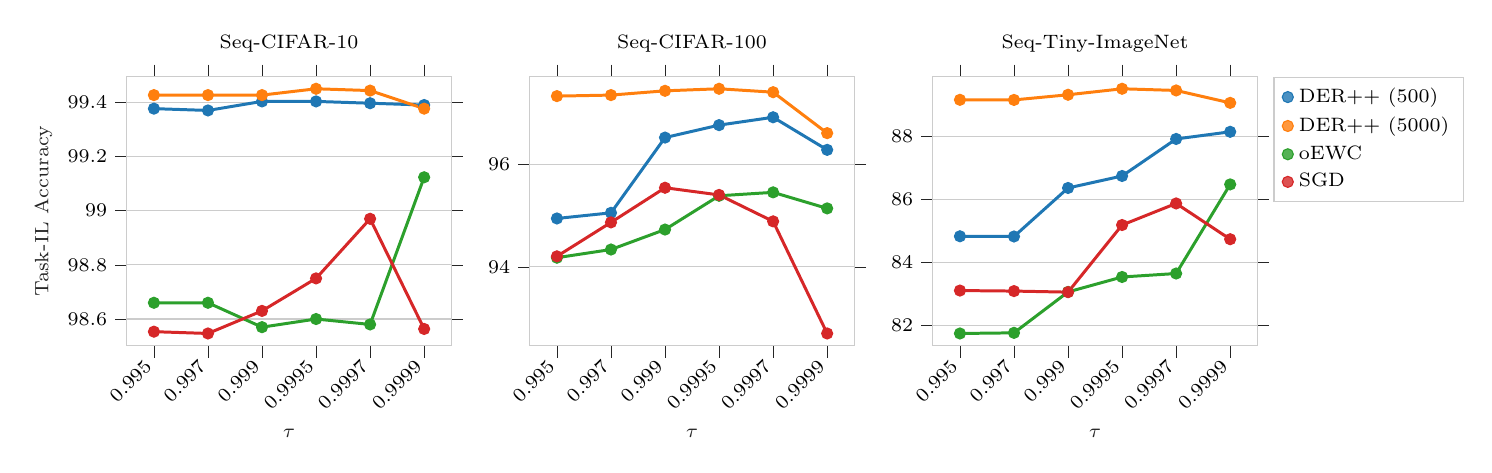
\begin{tikzpicture}
\scriptsize
\definecolor{crimson2143940}{RGB}{214,39,40}
\definecolor{darkorange25512714}{RGB}{255,127,14}
\definecolor{darkslategray38}{RGB}{38,38,38}
\definecolor{forestgreen4416044}{RGB}{44,160,44}
\definecolor{lightgray204}{RGB}{204,204,204}
\definecolor{steelblue31119180}{RGB}{31,119,180}

\begin{groupplot}[
    group style={group size=3 by 1},
    width=5.7cm,
    height=5cm
]
\nextgroupplot[
axis line style={lightgray204},
tick align=outside,
title={Seq-CIFAR-10},
unbounded coords=jump,
x grid style={lightgray204},
xlabel=\textcolor{darkslategray38}{$\tau$},
xmajorticks=true,
xmin=-0.5, xmax=5.5,
xtick style={color=darkslategray38},
xtick={0,1,2,3,4,5},
xticklabels={0.995,0.997,0.999,0.9995,0.9997,0.9999},
xticklabel style={rotate=45,anchor=east},
y grid style={lightgray204},
ylabel=\textcolor{darkslategray38}{Task-IL Accuracy},
ymajorgrids,
ymajorticks=true,
ymin=98.5015, ymax=99.4951666666667,
ytick style={color=darkslategray38}
]
\addplot [line width=1.08pt, steelblue31119180]
table {%
0 99.3766666666667
1 99.37
2 99.4033333333334
3 99.4033333333334
4 99.3966666666667
5 99.39
};
\addplot [line width=1.08pt, steelblue31119180]
table {%
0 nan
0 nan
};
\addplot [line width=1.08pt, steelblue31119180]
table {%
1 nan
1 nan
};
\addplot [line width=1.08pt, steelblue31119180]
table {%
2 nan
2 nan
};
\addplot [line width=1.08pt, steelblue31119180]
table {%
3 nan
3 nan
};
\addplot [line width=1.08pt, steelblue31119180]
table {%
4 nan
4 nan
};
\addplot [line width=1.08pt, steelblue31119180]
table {%
5 nan
5 nan
};
\addplot [draw=steelblue31119180, fill=steelblue31119180, mark=*, only marks]
table{%
x  y
0 99.3766666666667
1 99.37
2 99.4033333333334
3 99.4033333333334
4 99.3966666666667
5 99.39
};
\addplot [line width=1.08pt, darkorange25512714]
table {%
0 99.4266666666667
1 99.4266666666667
2 99.4266666666667
3 99.45
4 99.4433333333333
5 99.3766666666667
};
\addplot [line width=1.08pt, darkorange25512714]
table {%
0 nan
0 nan
};
\addplot [line width=1.08pt, darkorange25512714]
table {%
1 nan
1 nan
};
\addplot [line width=1.08pt, darkorange25512714]
table {%
2 nan
2 nan
};
\addplot [line width=1.08pt, darkorange25512714]
table {%
3 nan
3 nan
};
\addplot [line width=1.08pt, darkorange25512714]
table {%
4 nan
4 nan
};
\addplot [line width=1.08pt, darkorange25512714]
table {%
5 nan
5 nan
};
\addplot [draw=darkorange25512714, fill=darkorange25512714, mark=*, only marks]
table{%
x  y
0 99.4266666666667
1 99.4266666666667
2 99.4266666666667
3 99.45
4 99.4433333333333
5 99.3766666666667
};
\addplot [line width=1.08pt, forestgreen4416044]
table {%
0 98.66
1 98.66
2 98.57
3 98.6
4 98.58
5 99.1233333333333
};
\addplot [line width=1.08pt, forestgreen4416044]
table {%
0 nan
0 nan
};
\addplot [line width=1.08pt, forestgreen4416044]
table {%
1 nan
1 nan
};
\addplot [line width=1.08pt, forestgreen4416044]
table {%
2 nan
2 nan
};
\addplot [line width=1.08pt, forestgreen4416044]
table {%
3 nan
3 nan
};
\addplot [line width=1.08pt, forestgreen4416044]
table {%
4 nan
4 nan
};
\addplot [line width=1.08pt, forestgreen4416044]
table {%
5 nan
5 nan
};
\addplot [draw=forestgreen4416044, fill=forestgreen4416044, mark=*, only marks]
table{%
x  y
0 98.66
1 98.66
2 98.57
3 98.6
4 98.58
5 99.1233333333333
};
\addplot [line width=1.08pt, crimson2143940]
table {%
0 98.5533333333333
1 98.5466666666667
2 98.63
3 98.75
4 98.97
5 98.5633333333333
};
\addplot [line width=1.08pt, crimson2143940]
table {%
0 nan
0 nan
};
\addplot [line width=1.08pt, crimson2143940]
table {%
1 nan
1 nan
};
\addplot [line width=1.08pt, crimson2143940]
table {%
2 nan
2 nan
};
\addplot [line width=1.08pt, crimson2143940]
table {%
3 nan
3 nan
};
\addplot [line width=1.08pt, crimson2143940]
table {%
4 nan
4 nan
};
\addplot [line width=1.08pt, crimson2143940]
table {%
5 nan
5 nan
};
\addplot [draw=crimson2143940, fill=crimson2143940, mark=*, only marks]
table{%
x  y
0 98.5533333333333
1 98.5466666666667
2 98.63
3 98.75
4 98.97
5 98.5633333333333
};

\nextgroupplot[
axis line style={lightgray204},
tick align=outside,
title={Seq-CIFAR-100},
unbounded coords=jump,
x grid style={lightgray204},
xlabel=\textcolor{darkslategray38}{$\tau$},
xmajorticks=true,
xmin=-0.5, xmax=5.5,
xtick style={color=darkslategray38},
xtick={0,1,2,3,4,5},
xticklabels={0.995,0.997,0.999,0.9995,0.9997,0.9999},
xticklabel style={rotate=45,anchor=east},
y grid style={lightgray204},
ylabel=\textcolor{darkslategray38}{},
ymajorgrids,
ymajorticks=true,
ymin=92.461, ymax=97.719,
ytick style={color=darkslategray38}
]
\addplot [line width=1.08pt, steelblue31119180]
table {%
0 94.9466666666667
1 95.0566666666667
2 96.5266666666667
3 96.77
4 96.9233333333333
5 96.2866666666667
};
\addplot [line width=1.08pt, steelblue31119180]
table {%
0 nan
0 nan
};
\addplot [line width=1.08pt, steelblue31119180]
table {%
1 nan
1 nan
};
\addplot [line width=1.08pt, steelblue31119180]
table {%
2 nan
2 nan
};
\addplot [line width=1.08pt, steelblue31119180]
table {%
3 nan
3 nan
};
\addplot [line width=1.08pt, steelblue31119180]
table {%
4 nan
4 nan
};
\addplot [line width=1.08pt, steelblue31119180]
table {%
5 nan
5 nan
};
\addplot [draw=steelblue31119180, fill=steelblue31119180, mark=*, only marks]
table{%
x  y
0 94.9466666666667
1 95.0566666666667
2 96.5266666666667
3 96.77
4 96.9233333333333
5 96.2866666666667
};
\addplot [line width=1.08pt, darkorange25512714]
table {%
0 97.3366666666667
1 97.3566666666667
2 97.44
3 97.48
4 97.4133333333333
5 96.6133333333333
};
\addplot [line width=1.08pt, darkorange25512714]
table {%
0 nan
0 nan
};
\addplot [line width=1.08pt, darkorange25512714]
table {%
1 nan
1 nan
};
\addplot [line width=1.08pt, darkorange25512714]
table {%
2 nan
2 nan
};
\addplot [line width=1.08pt, darkorange25512714]
table {%
3 nan
3 nan
};
\addplot [line width=1.08pt, darkorange25512714]
table {%
4 nan
4 nan
};
\addplot [line width=1.08pt, darkorange25512714]
table {%
5 nan
5 nan
};
\addplot [draw=darkorange25512714, fill=darkorange25512714, mark=*, only marks]
table{%
x  y
0 97.3366666666667
1 97.3566666666667
2 97.44
3 97.48
4 97.4133333333333
5 96.6133333333333
};
\addplot [line width=1.08pt, forestgreen4416044]
table {%
0 94.18
1 94.34
2 94.73
3 95.39
4 95.4566666666667
5 95.1433333333333
};
\addplot [line width=1.08pt, forestgreen4416044]
table {%
0 nan
0 nan
};
\addplot [line width=1.08pt, forestgreen4416044]
table {%
1 nan
1 nan
};
\addplot [line width=1.08pt, forestgreen4416044]
table {%
2 nan
2 nan
};
\addplot [line width=1.08pt, forestgreen4416044]
table {%
3 nan
3 nan
};
\addplot [line width=1.08pt, forestgreen4416044]
table {%
4 nan
4 nan
};
\addplot [line width=1.08pt, forestgreen4416044]
table {%
5 nan
5 nan
};
\addplot [draw=forestgreen4416044, fill=forestgreen4416044, mark=*, only marks]
table{%
x  y
0 94.18
1 94.34
2 94.73
3 95.39
4 95.4566666666667
5 95.1433333333333
};
\addplot [line width=1.08pt, crimson2143940]
table {%
0 94.2066666666667
1 94.87
2 95.5466666666667
3 95.4066666666667
4 94.89
5 92.7
};
\addplot [line width=1.08pt, crimson2143940]
table {%
0 nan
0 nan
};
\addplot [line width=1.08pt, crimson2143940]
table {%
1 nan
1 nan
};
\addplot [line width=1.08pt, crimson2143940]
table {%
2 nan
2 nan
};
\addplot [line width=1.08pt, crimson2143940]
table {%
3 nan
3 nan
};
\addplot [line width=1.08pt, crimson2143940]
table {%
4 nan
4 nan
};
\addplot [line width=1.08pt, crimson2143940]
table {%
5 nan
5 nan
};
\addplot [draw=crimson2143940, fill=crimson2143940, mark=*, only marks]
table{%
x  y
0 94.2066666666667
1 94.87
2 95.5466666666667
3 95.4066666666667
4 94.89
5 92.7
};

\nextgroupplot[
axis line style={lightgray204},
legend cell align={left},
legend style={
  fill opacity=0.8,
  draw opacity=1,
  text opacity=1,
  at={(1.05,1)},
  anchor=north west,
  draw=lightgray204
},
tick align=outside,
title={Seq-Tiny-ImageNet},
unbounded coords=jump,
x grid style={lightgray204},
xlabel=\textcolor{darkslategray38}{$\tau$},
xmajorticks=true,
xmin=-0.5, xmax=5.5,
xtick style={color=darkslategray38},
xtick={0,1,2,3,4,5},
xticklabels={0.995,0.997,0.999,0.9995,0.9997,0.9999},
xticklabel style={rotate=45,anchor=east},
y grid style={lightgray204},
ylabel=\textcolor{darkslategray38}{},
ymajorgrids,
ymajorticks=true,
ymin=81.3623333333333, ymax=89.891,
ytick style={color=darkslategray38}
]
\addplot [line width=1.08pt, steelblue31119180, forget plot]
table {%
0 84.83
1 84.8233333333333
2 86.36
3 86.74
4 87.9133333333333
5 88.14
};
\addplot [line width=1.08pt, steelblue31119180, forget plot]
table {%
0 nan
0 nan
};
\addplot [line width=1.08pt, steelblue31119180, forget plot]
table {%
1 nan
1 nan
};
\addplot [line width=1.08pt, steelblue31119180, forget plot]
table {%
2 nan
2 nan
};
\addplot [line width=1.08pt, steelblue31119180, forget plot]
table {%
3 nan
3 nan
};
\addplot [line width=1.08pt, steelblue31119180, forget plot]
table {%
4 nan
4 nan
};
\addplot [line width=1.08pt, steelblue31119180, forget plot]
table {%
5 nan
5 nan
};
\addplot [draw=steelblue31119180, fill=steelblue31119180, mark=*, only marks]
table{%
x  y
0 84.83
1 84.8233333333333
2 86.36
3 86.74
4 87.9133333333333
5 88.14
};
\addlegendentry{DER++ (500)}
\addplot [line width=1.08pt, darkorange25512714, forget plot]
table {%
0 89.1533333333333
1 89.15
2 89.3133333333333
3 89.5033333333333
4 89.45
5 89.0566666666667
};
\addplot [line width=1.08pt, darkorange25512714, forget plot]
table {%
0 nan
0 nan
};
\addplot [line width=1.08pt, darkorange25512714, forget plot]
table {%
1 nan
1 nan
};
\addplot [line width=1.08pt, darkorange25512714, forget plot]
table {%
2 nan
2 nan
};
\addplot [line width=1.08pt, darkorange25512714, forget plot]
table {%
3 nan
3 nan
};
\addplot [line width=1.08pt, darkorange25512714, forget plot]
table {%
4 nan
4 nan
};
\addplot [line width=1.08pt, darkorange25512714, forget plot]
table {%
5 nan
5 nan
};
\addplot [draw=darkorange25512714, fill=darkorange25512714, mark=*, only marks]
table{%
x  y
0 89.1533333333333
1 89.15
2 89.3133333333333
3 89.5033333333333
4 89.45
5 89.0566666666667
};
\addlegendentry{DER++ (5000)}
\addplot [line width=1.08pt, forestgreen4416044, forget plot]
table {%
0 81.75
1 81.77
2 83.0666666666667
3 83.54
4 83.65
5 86.4733333333333
};
\addplot [line width=1.08pt, forestgreen4416044, forget plot]
table {%
0 nan
0 nan
};
\addplot [line width=1.08pt, forestgreen4416044, forget plot]
table {%
1 nan
1 nan
};
\addplot [line width=1.08pt, forestgreen4416044, forget plot]
table {%
2 nan
2 nan
};
\addplot [line width=1.08pt, forestgreen4416044, forget plot]
table {%
3 nan
3 nan
};
\addplot [line width=1.08pt, forestgreen4416044, forget plot]
table {%
4 nan
4 nan
};
\addplot [line width=1.08pt, forestgreen4416044, forget plot]
table {%
5 nan
5 nan
};
\addplot [draw=forestgreen4416044, fill=forestgreen4416044, mark=*, only marks]
table{%
x  y
0 81.75
1 81.77
2 83.0666666666667
3 83.54
4 83.65
5 86.4733333333333
};
\addlegendentry{oEWC}
\addplot [line width=1.08pt, crimson2143940, forget plot]
table {%
0 83.11
1 83.0933333333333
2 83.06
3 85.1866666666667
4 85.87
5 84.7366666666667
};
\addplot [line width=1.08pt, crimson2143940, forget plot]
table {%
0 nan
0 nan
};
\addplot [line width=1.08pt, crimson2143940, forget plot]
table {%
1 nan
1 nan
};
\addplot [line width=1.08pt, crimson2143940, forget plot]
table {%
2 nan
2 nan
};
\addplot [line width=1.08pt, crimson2143940, forget plot]
table {%
3 nan
3 nan
};
\addplot [line width=1.08pt, crimson2143940, forget plot]
table {%
4 nan
4 nan
};
\addplot [line width=1.08pt, crimson2143940, forget plot]
table {%
5 nan
5 nan
};
\addplot [draw=crimson2143940, fill=crimson2143940, mark=*, only marks]
table{%
x  y
0 83.11
1 83.0933333333333
2 83.06
3 85.1866666666667
4 85.87
5 84.7366666666667
};
\addlegendentry{SGD}
\end{groupplot}

\end{tikzpicture}

%     \vspace{-1cm}
%     \caption{The effect of the hyper-parameter $\tau$ on the Task-IL Accuracy}%
%     \label{fig:tau_task-il-acc}%
% \end{figure*}

\begin{figure*}[ht!]
    \centering
    % This file was created with tikzplotlib v0.10.1.
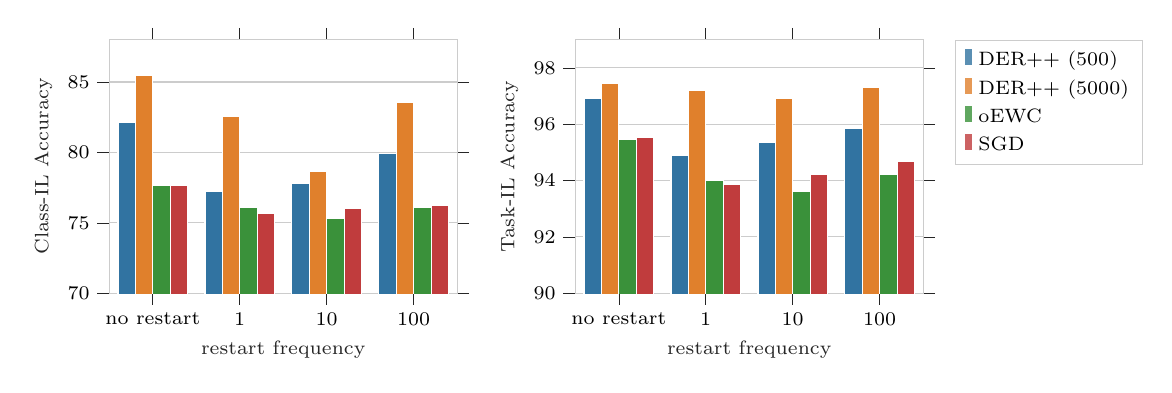
\begin{tikzpicture}
\scriptsize

\definecolor{brown1926061}{RGB}{192,60,61}
\definecolor{darkslategray38}{RGB}{38,38,38}
\definecolor{darkslategray66}{RGB}{66,66,66}
\definecolor{lightgray204}{RGB}{204,204,204}
\definecolor{peru22412844}{RGB}{224,128,44}
\definecolor{seagreen5814558}{RGB}{58,145,58}
\definecolor{steelblue49115161}{RGB}{49,115,161}

\begin{groupplot}[
    group style={group size=2 by 1},
    width=6cm,
    height=4.8cm
]

\nextgroupplot[
axis line style={lightgray204},
legend cell align={left},
legend style={
  fill opacity=0.8,
  draw opacity=1,
  text opacity=1,
  at={(2.43,1)},
  anchor=north west,
  draw=lightgray204
},
tick align=outside,
unbounded coords=jump,
x grid style={lightgray204},
xlabel=\textcolor{darkslategray38}{restart frequency},
xmajorticks=true,
xmin=-0.5, xmax=3.5,
xtick style={color=darkslategray38},
xtick={0,1,2,3},
xticklabels={\text{no restart},1,10,100},
y grid style={lightgray204},
ylabel=\textcolor{darkslategray38}{Class-IL Accuracy},
ymajorgrids,
ymajorticks=true,
ymin=70, ymax=88,
ytick style={color=darkslategray38}
]
\draw[draw=white,fill=steelblue49115161] (axis cs:-0.4,0) rectangle (axis cs:-0.2,82.14);
\addlegendimage{ybar,ybar legend,draw=white,fill=steelblue49115161}
\addlegendentry{DER++ (500)}

\draw[draw=white,fill=steelblue49115161] (axis cs:0.6,0) rectangle (axis cs:0.8,77.1933333333333);
\draw[draw=white,fill=steelblue49115161] (axis cs:1.6,0) rectangle (axis cs:1.8,77.77);
\draw[draw=white,fill=steelblue49115161] (axis cs:2.6,0) rectangle (axis cs:2.8,79.9433333333333);
\draw[draw=white,fill=peru22412844] (axis cs:-0.2,0) rectangle (axis cs:0,85.4533333333333);
\addlegendimage{ybar,ybar legend,draw=white,fill=peru22412844}
\addlegendentry{DER++ (5000)}

\draw[draw=white,fill=peru22412844] (axis cs:0.8,0) rectangle (axis cs:1,82.5866666666667);
\draw[draw=white,fill=peru22412844] (axis cs:1.8,0) rectangle (axis cs:2,78.6533333333333);
\draw[draw=white,fill=peru22412844] (axis cs:2.8,0) rectangle (axis cs:3,83.53);
\draw[draw=white,fill=seagreen5814558] (axis cs:2.77555756156289e-17,0) rectangle (axis cs:0.2,77.6633333333333);
\addlegendimage{ybar,ybar legend,draw=white,fill=seagreen5814558}
\addlegendentry{oEWC}

\draw[draw=white,fill=seagreen5814558] (axis cs:1,0) rectangle (axis cs:1.2,76.0933333333333);
\draw[draw=white,fill=seagreen5814558] (axis cs:2,0) rectangle (axis cs:2.2,75.3066666666667);
\draw[draw=white,fill=seagreen5814558] (axis cs:3,0) rectangle (axis cs:3.2,76.07);
\draw[draw=white,fill=brown1926061] (axis cs:0.2,0) rectangle (axis cs:0.4,77.6633333333333);
\addlegendimage{ybar,ybar legend,draw=white,fill=brown1926061}
\addlegendentry{SGD}

\draw[draw=white,fill=brown1926061] (axis cs:1.2,0) rectangle (axis cs:1.4,75.67);
\draw[draw=white,fill=brown1926061] (axis cs:2.2,0) rectangle (axis cs:2.4,76.0233333333333);
\draw[draw=white,fill=brown1926061] (axis cs:3.2,0) rectangle (axis cs:3.4,76.2);
\addplot [line width=1.08pt, darkslategray66]
table {%
-0.3 nan
-0.3 nan
};
\addplot [line width=1.08pt, darkslategray66]
table {%
0.7 nan
0.7 nan
};
\addplot [line width=1.08pt, darkslategray66]
table {%
1.7 nan
1.7 nan
};
\addplot [line width=1.08pt, darkslategray66]
table {%
2.7 nan
2.7 nan
};
\addplot [line width=1.08pt, darkslategray66]
table {%
-0.1 nan
-0.1 nan
};
\addplot [line width=1.08pt, darkslategray66]
table {%
0.9 nan
0.9 nan
};
\addplot [line width=1.08pt, darkslategray66]
table {%
1.9 nan
1.9 nan
};
\addplot [line width=1.08pt, darkslategray66]
table {%
2.9 nan
2.9 nan
};
\addplot [line width=1.08pt, darkslategray66]
table {%
0.1 nan
0.1 nan
};
\addplot [line width=1.08pt, darkslategray66]
table {%
1.1 nan
1.1 nan
};
\addplot [line width=1.08pt, darkslategray66]
table {%
2.1 nan
2.1 nan
};
\addplot [line width=1.08pt, darkslategray66]
table {%
3.1 nan
3.1 nan
};
\addplot [line width=1.08pt, darkslategray66]
table {%
0.3 nan
0.3 nan
};
\addplot [line width=1.08pt, darkslategray66]
table {%
1.3 nan
1.3 nan
};
\addplot [line width=1.08pt, darkslategray66]
table {%
2.3 nan
2.3 nan
};
\addplot [line width=1.08pt, darkslategray66]
table {%
3.3 nan
3.3 nan
};

\nextgroupplot[
axis line style={lightgray204},
xshift=0.5cm,
tick align=outside,
unbounded coords=jump,
x grid style={lightgray204},
xlabel=\textcolor{darkslategray38}{restart frequency},
xmajorticks=true,
xmin=-0.5, xmax=3.5,
xtick style={color=darkslategray38},
xtick={0,1,2,3},
xticklabels={\text{no restart},1,10,100},
y grid style={lightgray204},
ylabel=\textcolor{darkslategray38}{Task-IL Accuracy},
ymajorgrids,
ymajorticks=true,
ymin=90, ymax=99,
ytick style={color=darkslategray38}
]
\draw[draw=white,fill=steelblue49115161] (axis cs:-0.4,0) rectangle (axis cs:-0.2,96.9233333333333);
\draw[draw=white,fill=steelblue49115161] (axis cs:0.6,0) rectangle (axis cs:0.8,94.9033333333333);
\draw[draw=white,fill=steelblue49115161] (axis cs:1.6,0) rectangle (axis cs:1.8,95.3466666666667);
\draw[draw=white,fill=steelblue49115161] (axis cs:2.6,0) rectangle (axis cs:2.8,95.8433333333333);
\draw[draw=white,fill=peru22412844] (axis cs:-0.2,0) rectangle (axis cs:0,97.44);
\draw[draw=white,fill=peru22412844] (axis cs:0.8,0) rectangle (axis cs:1,97.2166666666667);
\draw[draw=white,fill=peru22412844] (axis cs:1.8,0) rectangle (axis cs:2,96.93);
\draw[draw=white,fill=peru22412844] (axis cs:2.8,0) rectangle (axis cs:3,97.32);
\draw[draw=white,fill=seagreen5814558] (axis cs:2.77555756156289e-17,0) rectangle (axis cs:0.2,95.4566666666667);
\draw[draw=white,fill=seagreen5814558] (axis cs:1,0) rectangle (axis cs:1.2,93.9966666666667);
\draw[draw=white,fill=seagreen5814558] (axis cs:2,0) rectangle (axis cs:2.2,93.6133333333333);
\draw[draw=white,fill=seagreen5814558] (axis cs:3,0) rectangle (axis cs:3.2,94.2233333333333);
\draw[draw=white,fill=brown1926061] (axis cs:0.2,0) rectangle (axis cs:0.4,95.5466666666667);
\draw[draw=white,fill=brown1926061] (axis cs:1.2,0) rectangle (axis cs:1.4,93.86);
\draw[draw=white,fill=brown1926061] (axis cs:2.2,0) rectangle (axis cs:2.4,94.2166666666667);
\draw[draw=white,fill=brown1926061] (axis cs:3.2,0) rectangle (axis cs:3.4,94.6766666666667);
\addplot [line width=1.08pt, darkslategray66, forget plot]
table {%
-0.3 nan
-0.3 nan
};
\addplot [line width=1.08pt, darkslategray66, forget plot]
table {%
0.7 nan
0.7 nan
};
\addplot [line width=1.08pt, darkslategray66, forget plot]
table {%
1.7 nan
1.7 nan
};
\addplot [line width=1.08pt, darkslategray66, forget plot]
table {%
2.7 nan
2.7 nan
};
\addplot [line width=1.08pt, darkslategray66, forget plot]
table {%
-0.1 nan
-0.1 nan
};
\addplot [line width=1.08pt, darkslategray66, forget plot]
table {%
0.9 nan
0.9 nan
};
\addplot [line width=1.08pt, darkslategray66, forget plot]
table {%
1.9 nan
1.9 nan
};
\addplot [line width=1.08pt, darkslategray66, forget plot]
table {%
2.9 nan
2.9 nan
};
\addplot [line width=1.08pt, darkslategray66, forget plot]
table {%
0.1 nan
0.1 nan
};
\addplot [line width=1.08pt, darkslategray66, forget plot]
table {%
1.1 nan
1.1 nan
};
\addplot [line width=1.08pt, darkslategray66, forget plot]
table {%
2.1 nan
2.1 nan
};
\addplot [line width=1.08pt, darkslategray66, forget plot]
table {%
3.1 nan
3.1 nan
};
\addplot [line width=1.08pt, darkslategray66, forget plot]
table {%
0.3 nan
0.3 nan
};
\addplot [line width=1.08pt, darkslategray66, forget plot]
table {%
1.3 nan
1.3 nan
};
\addplot [line width=1.08pt, darkslategray66, forget plot]
table {%
2.3 nan
2.3 nan
};
\addplot [line width=1.08pt, darkslategray66, forget plot]
table {%
3.3 nan
3.3 nan
};
\end{groupplot}

\end{tikzpicture}

    \vspace{-1cm}
    \caption{The effect of restarting the fast weights with the slow weights at various restart frequencies. }%
    \label{fig:restats}%
\end{figure*}

\begin{figure*}[ht!]
    \centering
    \include{figures/update_freq-acc.tex}
    \vspace{-1cm}
    \caption{The effect of computing the momentum update at various update  frequencies.}%
    \label{fig:updates}%
\end{figure*}

%%%%%%%%%%%%%%%%%%%%%%%%%%%%%%%%%%%%%%%%%%%%%%%%%%%%%%%%%%%%%%%%%%%%%%%%
%%%%%%%%%%%%%%%%%%%%%%%%%%%%%%%%%%%%%%%%%%%%%%%%%%%%%%%%%%%%%%%%%%%%%%%%
\section{Conclusion}
Placeholder. Placeholder.

%%%%%%%%% REFERENCES
{\small
\bibliographystyle{ieee_fullname}
\bibliography{main}
}

\end{document}
